96. \begin{figure}[ht!]
\center{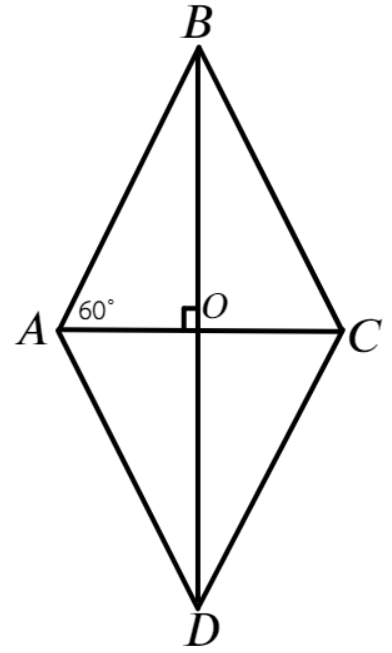
\includegraphics[scale=0.35]{g8-96.png}}
\end{figure}\\
В ромбе диагонали перпендикулярны и являются биссектрисами его углов, поэтому треугольник $ABO$ является прямоугольным и $\angle BAO=120^\circ:2=60^\circ.$ Тогда $AO=AB\cos(60^\circ)=20\cdot\cfrac{1}{2}=10.$\\
